\section{IPM prototype Simulations}
\subsection{Project overview}
\begin{frame}
  \frametitle{Project overview}
  \begin{block}{Project in brief}
    Provide 5 pairs of IPMs for the superconducting part of the ESS accelerator.
    \begin{itemize}
      \item In-Kind collaboration between CEA/IRFU and ESS
      \item Around XX peoples involved
    \end{itemize}
  \end{block}
  \begin{block}{Project milestones}
    \begin{itemize}
      \item[2016] Kick-off meeting (April), beginning of my PhD (October)
      \item[2017] Preliminary Design Review (February), simulations, design and manufacturing
      \item[2018] \underline{Mainly beam tests and data analysis}
      \item[2019] Critical Design Review (March), design and manufacturing of final IPMs, end of my PhD (October)
      \item[2020] First IPM delivery, Handover 
    \end{itemize}
  \end{block}
\end{frame}

\begin{frame}
  \frametitle{Requierements}
  \begin{block}{L4 requierements}
    ESS has specified some crucial requirements for the profilers.
    \begin{itemize}
      \item Measurement per pulse at nominal conditions
      \item Maximum error on the beam size $<\,10\,\%$
      \item 
    \end{itemize}
  \end{block}
  \begin{block}{Other requierements}
    ESS has specified some crucial requirements for their diagnostics.
    \begin{itemize}
      \item Compliant to the use of superconductive cavities nearby
      \item Restricted environnement
    \end{itemize}
  \end{block}
\end{frame}

\begin{frame}
  \frametitle{IPM}
  \begin{columns}
    \begin{column}{0.45\textwidth}
      \begin{block}{How it works}
        \begin{itemize}
          \item Quantification of the "primary" ionization signal.
          \item Determination of the $e^-$/ion trajectories during the drift.
          \item The choice of an efficient readout technology.
        \end{itemize}   
      \end{block}
    \end{column}
    \begin{column}{0.45\textwidth}
      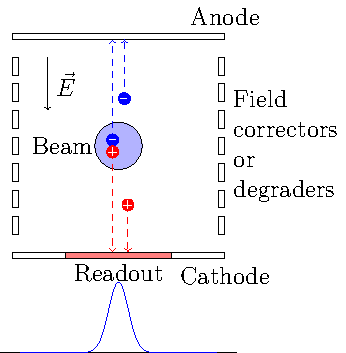
\includegraphics[width=\textwidth]{02_ESS/fig/fig000_IPM.pdf}
    \end{column}
  \end{columns}
\end{frame}

\subsection{Primary ionization signal}
\begin{frame}
  \frametitle{Primary ionization signal}

\end{frame}

\subsection{Field uniformity}
\begin{frame}
  \frametitle{Field uniformity}

\end{frame}

\begin{frame}
  \frametitle{Field uniformity}

\end{frame}

\subsection{Space charge}
\begin{frame}
  \frametitle{Space charge}

\end{frame}

\begin{frame}
  \frametitle{Space charge}

\end{frame}

\subsection{Readout}
\begin{frame}
  \frametitle{Strip}

\end{frame}

\begin{frame}
  \frametitle{MCP}

\end{frame}

\begin{frame}
  \frametitle{Silicon}

\end{frame}